\chapter{Czujnik ciśnienia atmosferycznego BMP085}
Czujnik ten jest wysoce precyzyjnym, cyfrowym czujnikiem ciśnienia oraz temperatury powietrza. Jego energooszczędność oraz niskie zapotrzebowanie na zasilanie napięciem (do 3,6 V) sprawia, że jest idealnym rozwiązaniem do zastosować w urządzeniach codzienniego użytku, tak jak telefony komórkowe, nawigacje GPS. Dzięki bardzo szybkiemu czasu przetwarzania danych (do 7,5 ms) oraz niskiemu wpływu zakłóceń daje najlepsze rezultaty.


BMP085 jest często używany w prognozowaniu pogody, ze względu na obecność dwóch czujników (ciśnienia i temperatury). Można go również wykorzystać do wyznaczenia wysokości względnej oraz bezwzględnej. W tym celu używane jest prawo zależności wysokości od ciśnienia, tzw. wzór barometryczny:
$$ p = p_{0} * exp(-\frac{\mu g h}{RT}) $$


Czujnik jest 
\begin{figure}[h]
\centering
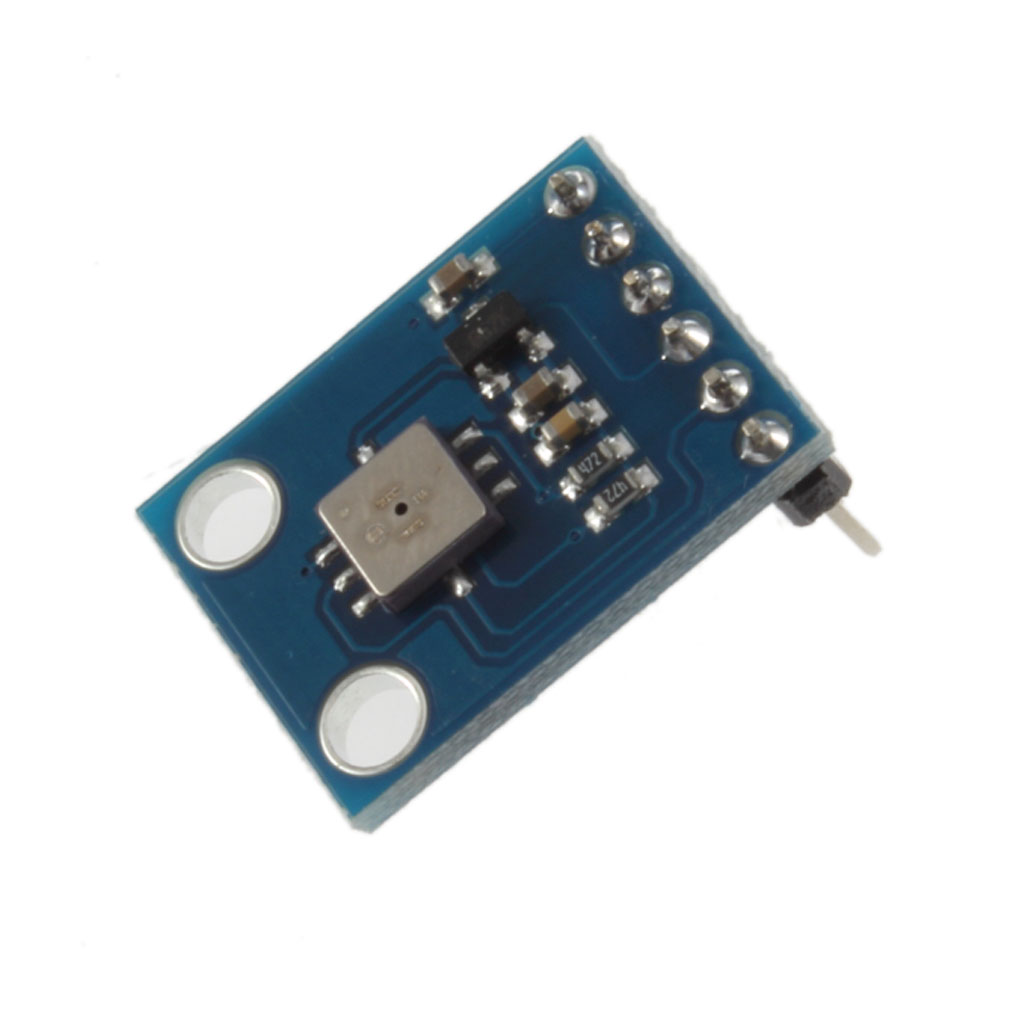
\includegraphics{bmp085_dol}
\caption{Czujnik ciśnienia BMP085 - widok z dołu}
\label{fig:bmp085_dol}
\end{figure}

\begin{figure}[h]
\centering
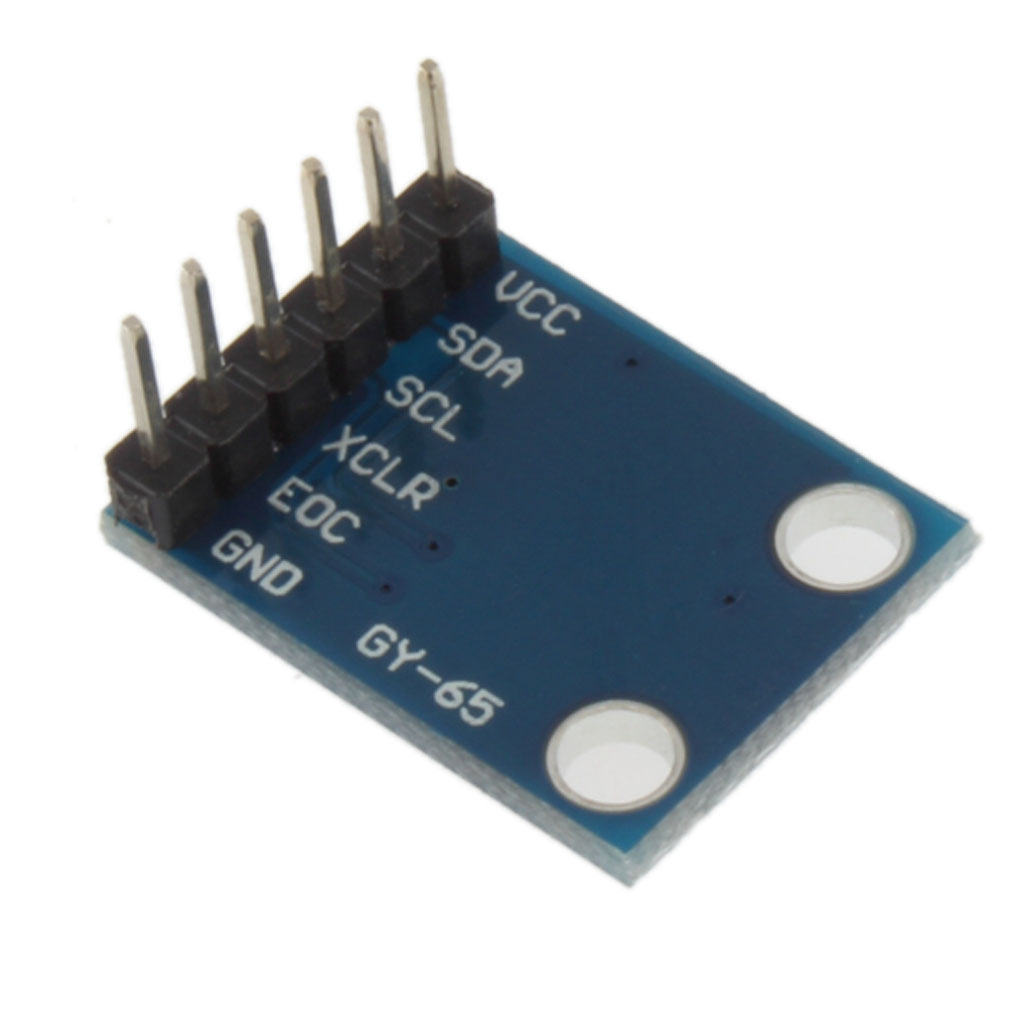
\includegraphics{bmp085_gora}
\caption{Czujnik ciśnienia BMP085 - widok z góry}
\label{fig:bmp085_gora}
\end{figure}